%%%%%%%%%%%%%%%%%%%%%%%%%%%%%%%%%%%%%%%%%%%%%%%%%%%%%%%%%%%%%%%%%%%%
% Grundlagen
%%%%%%%%%%%%%%%%%%%%%%%%%%%%%%%%%%%%%%%%%%%%%%%%%%%%%%%%%%%%%%%%%%%%
\chapter{Preliminaries}
  \label{PR}
This chapter introduces terms and definitions used in this thesis. \autoref{basics} explains what a graph is in graph theory and what attributes and structural properties a graph can have.
\autoref{LL} gives an introduction to linear layouts and distinguishes the different characteristics of linear layouts.
\autoref{SAT} provides the reader with a short introduction to SAT. 
\section{Basics}
\label{basics}
Formally a graph\index{Graph} $G = (V, E)$ consists of a finite set of vertices $V$ and a finite set of edges $E \subseteq V \times V$, where each edge $e_i$ connects two vertices $v_j, v_k \in V$. We state that $n := |V|$ and $m := |E|$.\\
A \textit{path}\index{Path} $p$ is a series of edges $(e_1, e_2,...,e_m)$, where $e_1,...,e_m \in E$. The same path can also be described as a sequence of vertices $(v_1,v_2,...,v_{m-1})$, where  $e_i$ connects $v_i$ to $v_{i+1}$.
\subsection{Attributes of a graph}
\subsubsection{Directed or undirected}
A graph can be either \textit{directed}\index{Directed graph} or \textit{undirected}.\\
In a \textit{directed} graph all edges $e \in E$ are described as ordered pairs of vertices $e = (u,v)$, where the first vertex is referred to as the source and the second is referred to as the target vertex.\\
In an \textit{undirected} graph each edge is defined by an unordered pair of vertices $e = \{u,v\}$ with no definite source or target. 
\subsubsection{Weighted or unweighted}
A graph can have \textit{weighted} \index{Weighted graph} or \textit{unweighted} edges.\\
If a graph is \textit{weighted} its definition includes a map $w: E \rightarrow \mathbb{R}$ which assigns a weight $w(e)$ to each edge $e \in E$. 
\subsection{Structural properties of a graph}
\subsubsection{Complete} 
\index{Complete graph}
A \textit{complete} graph contains an edge $e$ for every pair of vertices $v, u \in V$. \textit{Complete} graphs are denoted as $K_n$ where $n = |V|$.\\
A \textit{directed} complete graph with $n$ vertices has exactly $n^2$ edges, whereas an \textit{undirected} complete graph has $\frac{n^2 -n}{2}$ edges. The complete graphs $K_4$ and $K_5$ can be seen in \autoref{PPG}.
\subsubsection{Connected}
\index{Connected graph}
A graph is called \textit{connected}, if for every two vertices $v_i, v_j \in V$ there is a path from $v_i$ to $v_j$, meaning that there are no unreachable vertices (see in \autoref{img:COAC}a, where vertex 5 is unreachable).
\subsubsection{Acyclic}
\index{Acyclic graph}
An \textit{acyclic} graph has no cycles, which means that there exists no path $(v_0, v_1,...,v_k)$ where $v_0 = v_k$, that is to say that for every path in the graph the start vertex and the end vertex cannot be the same (see in \autoref{img:COAC}b).
\subsubsection{Trees and forests}
\index{Tree} \index{Forest}
A \textit{tree} is a \textit{connected}, \textit{acyclic} graph.\\
A \textit{forest} is a graph consisting of several tree graphs, meaning it is not \textit{connected} but still \textit{acyclic} (see \autoref{BTF}b and c).
\begin{figure}[h!]
\begin{center}
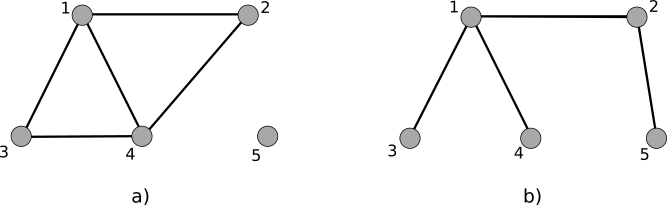
\includegraphics[width= \textwidth]{figures/ConnectedAcyclic.png}
\caption{Connectivity and acyclicity: a) neither connected nor acyclic graph b) connected and acyclic graph, also known as a \textit{tree}}
\label{img:COAC}
\end{center}
\end{figure}
\subsubsection{Bipartite}
\index{Bipartite graph}
A graph is called \textit{bipartite} if its vertex set $V$ can be partition in two disjoint subsets $V_0, V_1 \subset V$ such that $V_0 \cup V_1 = V$, $V_0 \cap V_1 = \emptyset$, and each edge $(u,v) \in E$ connects one vertex from $V_0$ with one vertex from $V_1$ (see in \autoref{BTF}a).\\

\begin{figure}[h!]
\begin{center}
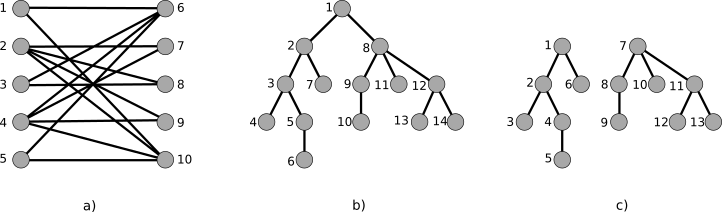
\includegraphics[width= \textwidth]{figures/BipartiteTreeForest.png}
\caption{Different graphs a) A bipartite graph, b) a tree, c) a forest}
\label{BTF}
\end{center}
\end{figure}

\subsubsection{Planarity}
\index{Planar graph}
A graph is \textit{planar} if it can be drawn on the plane such that no two edges $e_i, e_j \in E$ cross.\\
A graph is \textit{maximal planar} \index{Maximal planar graph} if no edge can be added to the graph without loosing planarity. $K_4$ is the biggest \textit{complete} graph that is planar.\\
A drawing of a graph is referred to as \textit{planar} if no edges cross. Note that a graph can be \textit{planar} but a particular drawing of the graph can be non-planar (see \autoref{PPG}).
\begin{figure}[h!]
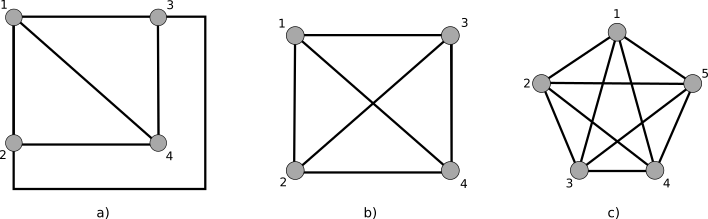
\includegraphics[width =\textwidth]{figures/PlanarPlaneGraphs.png}
\caption{On planarity a) $K_4$, planar graph and plane drawing, b) $K_4$, planar graph but non-planar drawing, c) $K_5$, neither planar graph nor planar drawing}
\label{PPG}
\end{figure}\\
A \textit{planar} drawing of a \textit{planar} graph defines several topologically connected regions which are called faces. The inner faces of a graph are regions enclosed by edges. The outer face of a graph is infinitely large and corresponds to the region outside the graph, bounded by its outer edges.\\
\index{Outerplanar graph}
\noindent A graph is called \textit{outerplanar}, when there exists a drawing in which all of its vertices belong to the outer face of the graph.
\section{Linear layouts}
\label{LL}
\index{Linear layout}
A linear layout of a graph is a drawing in which all the vertices $V$ are positioned along a line called the \textit{spine}.\\
The order in which these vertices are placed on the spine, is described by a bijective function $$\sigma : V \mapsto \{1,...,n\} $$ This function defines a relation where the following statements hold:
\begin{itemize}
\item Reflexivity: $\forall v_0 \in V: \sigma(v_0) \leq \sigma(v_0)$
\item Antisymmetry: $\sigma(v_0) \leq \sigma(v_1)$ and $\sigma(v_1) \leq \sigma(v_0)$ implies that $v_0 = v_1$
\item Transitivity: if $\sigma(v_0) \leq \sigma(v_1)$ and $\sigma(v_1) \leq \sigma(v_2)$ then $\sigma(v_0) \leq \sigma(v_2)$
\item Comparability: $\forall v_0, v_1 \in V$: either $\sigma(v_0) \leq \sigma(v_1)$ or $\sigma(v_1) \leq \sigma(v_0)$ is true
\end{itemize}
These properties make the relation a \textit{total order} \index{Total order} and the set of vertices a \textit{linearly ordered set}.\\
The edges of the graph are partitioned into $p$ disjoint subsets $E_p \subseteq E$ by the surjective function 
$$ \pi: E \rightarrow \{1,..,p\} $$ making $\pi$ a partition of $E$.\\
These subsets are called \textit{pages} of the linear layout. Each page represents one half-plane, delimited by the spine on which all the edges assigned to this subset will be placed.
In order to make it possible to draw these graphs in a 2D setting the edges of a half-plane are often colored which is why the half planes are sometimes also referred to as \textit{colors}.\\
The following sections explain which requirements the order of vertices and the assignment of edges follow.
\begin{figure}[!h]
\begin{center}
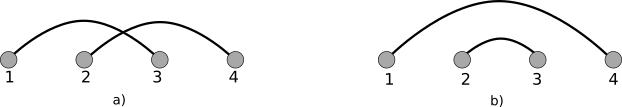
\includegraphics[width=1\textwidth]{figures/CrossingNesting.png}
\caption{Edges a) crossing edges, b) nesting edges}
\label{img:crossNest}
\end{center}
\end{figure}
\subsection{Stack layouts}
\index{Stack layout}
For a stack layout $\mathcal{E}(G,p)$, sometimes also referred to as a \textit{book embedding} \index{Book embedding}, the vertices $V$ need to be ordered in a way that no two edges $e_i, e_j$ assigned to the same subset, that is $\pi(e_i) = \pi(e_j)$, cross (see \autoref{img:crossNest}). In other words each half plane contains an \textit{outerplanar} subgraph. The subsets $E_p$ in a stack layout are called \textit{stacks}.\\
The \textit{book thickness} or \textit{stack number} \index{Stack number} \index{Book thickness} of a graph is the minimum number of pages that is needed to embed the graph.\\
In 1986 Yannakakis \cite{yannakakis1986four} proved that every planar graph admits  a stack layout with $p \leq 4$ pages. Yannakakis also sketched a construction of a graph with book thickness $p = 4$. However, his sketch was never completed and to this day researchers have not been able to prove the existence of a graph that requires four pages (see further explanation in \autoref{POC}).
\begin{figure}[!h]
\begin{center}
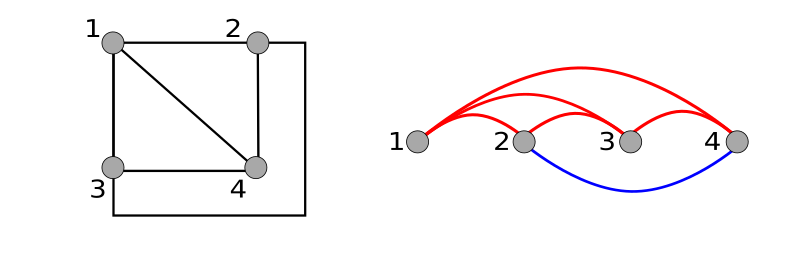
\includegraphics[width=0.7\textwidth]{figures/K4Stack.png}
\caption{$K_4$ and a corresponding 2-stack layout}
\label{img:stackGHG}
\end{center}
\end{figure}
\subsection{Queue layouts}
\index{Queue layout}
For a queue layout $\mathcal{Q}(G,q)$ the order of the vertices is chosen such that no two edges $e_i, e_j$ on the same pages are nested. Two edges $e_i, e_j$ are nested if both endpoints of edge $e_i$ are between both endpoints of edge $e_j$ (see \autoref{img:crossNest}). This property is not violated if edges $e_i, e_j$ share a common end vertex.
Similar to the \textit{book thickness} a graph has a \textit{queue number} \index{Queue number} that is defined as the minimum number of queues that are needed by any of its queue layouts.\\
As mentioned in the introdurction, the upper bound for the queue number of planar graphs is $49$ \cite{duj19}.
\begin{figure}[!h]
\begin{center}
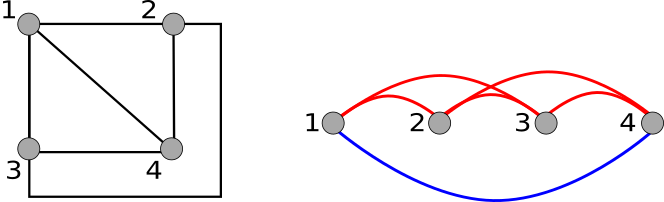
\includegraphics[width=0.7\textwidth]{figures/K4Queue.png}
\caption{$K_4$ and a corresponding queue layout}
\label{img:queueK4}
\end{center}
\end{figure}
\subsection{Further restrictions}
In addition to either being a stack or a queue, each page of a linear layout can be restricted further to have a special structure.
\subsubsection{Tree or forest subgraphs}
\index{Tree} \index{Forest}
A page of the layout has to be in the structure of a \textit{tree} or \textit{forest}, meaning that it is \textit{acyclic} and in the case of a \textit{tree} also \textit{connected}.
\subsubsection{Dispersable subgraphs}
\index{Dispersable subgraph}
A \textit{dispersable} subgraph is a graph in which no two edges share one endpoint. This kind of graph is also called a \textit{matching} \cite{kaufmann2018dispersable}. 
\begin{figure}[h!]
\begin{center}
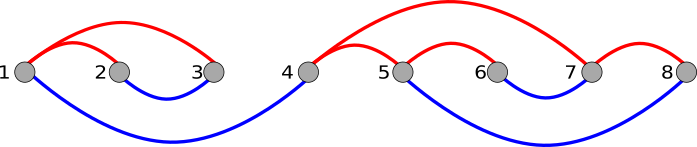
\includegraphics[width=1\textwidth]{figures/ForestDisp.png}
\caption{A linear layout with one forest stack (red) and one dispersable stack (blue)}
\label{img:layoutForestDisp}
\end{center}
\end{figure} 
\section{SAT}
\label{SAT}
In 2015 members of Algorithms Research Group of University of Tübingen proposed a new method to compute linear layouts automatically \cite{Bekos2015TheBE}, by formulating the problems as an instance of SAT which can then be solved with standard SAT solving techniques.\\
SAT \index{SAT} is short for satisfiability and means the Boolean satisfiability problem, which is the problem of determining whether there exists an assignment of truth values that satisfies a Boolean formula.
A logical formula for SAT is in \textit{conjunctive normal form} \index{Conjunctive normal form}, that means it is a conjunction (and, $\land$) of clauses or literals, and the clauses are disjunctions (or, $\lor$) of literals.\\
Most SAT-Solvers use a nondeterministic algorithm, that means for the same instance they can return different solutions.\\
For a detailed explanation of this refer to \cite{Bekos2015TheBE, jess}. The translation of the graph to a SAT instance is executed on \url{
http://alice.informatik.uni-tuebingen.de:5555/}.
